\section*{\begin{center}{Appendix E}\end{center}}
\addcontentsline{toc}{section}{Appendix E}
%$\\[0.5cm]$

\section*{Further experiment results}

\begin{figure}
    \centering
    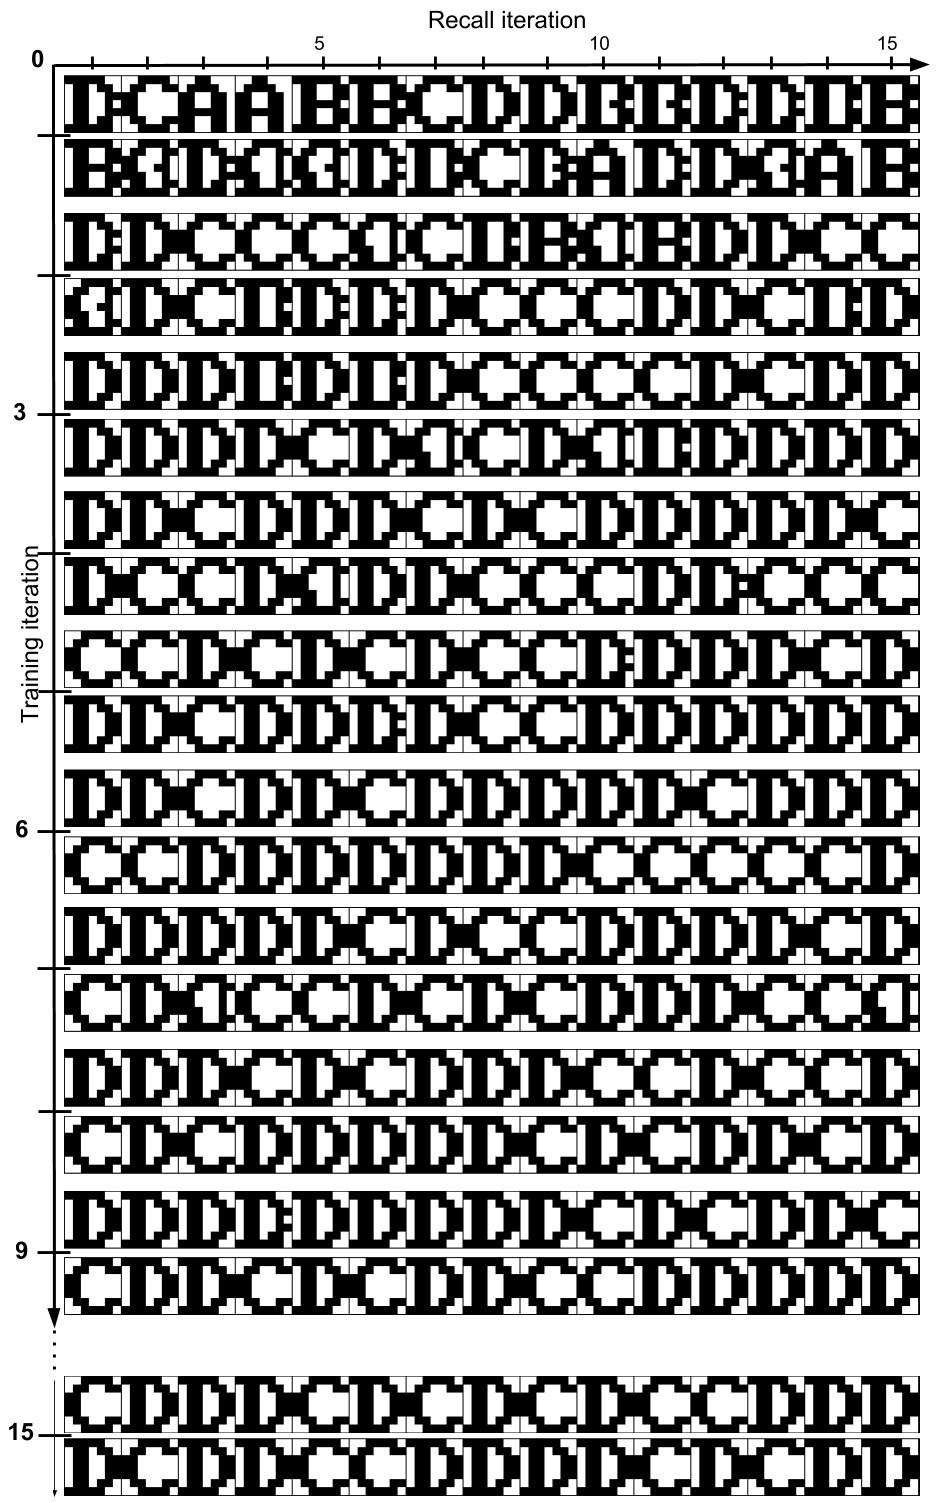
\includegraphics[width=11cm]{fig/CD-pattern-associations-async-tm0-dgw1-tau050}
    \caption{recall. async tm0 dgw1 tau050}
\end{figure}

\begin{figure}
    \centering
    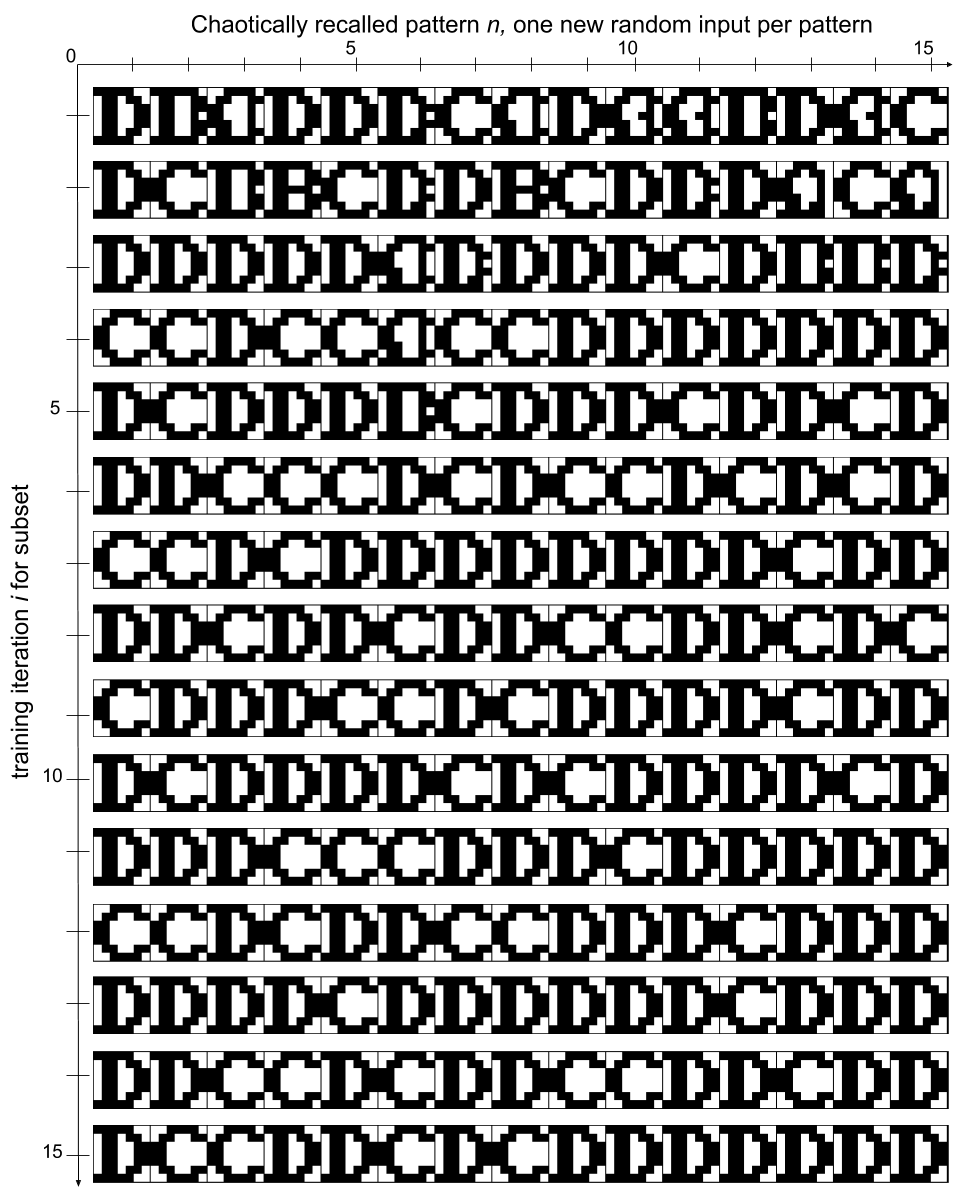
\includegraphics[width=12cm]{fig/CD-chaotic-recall-async-tm0-dgw1-tau050}
    \caption{chaotic recall. async tm0 dgw1 tau050}
\end{figure}

\subsection*{Further figures from experiment 4.2, DG-weighting}

\begin{figure}
    \centering
    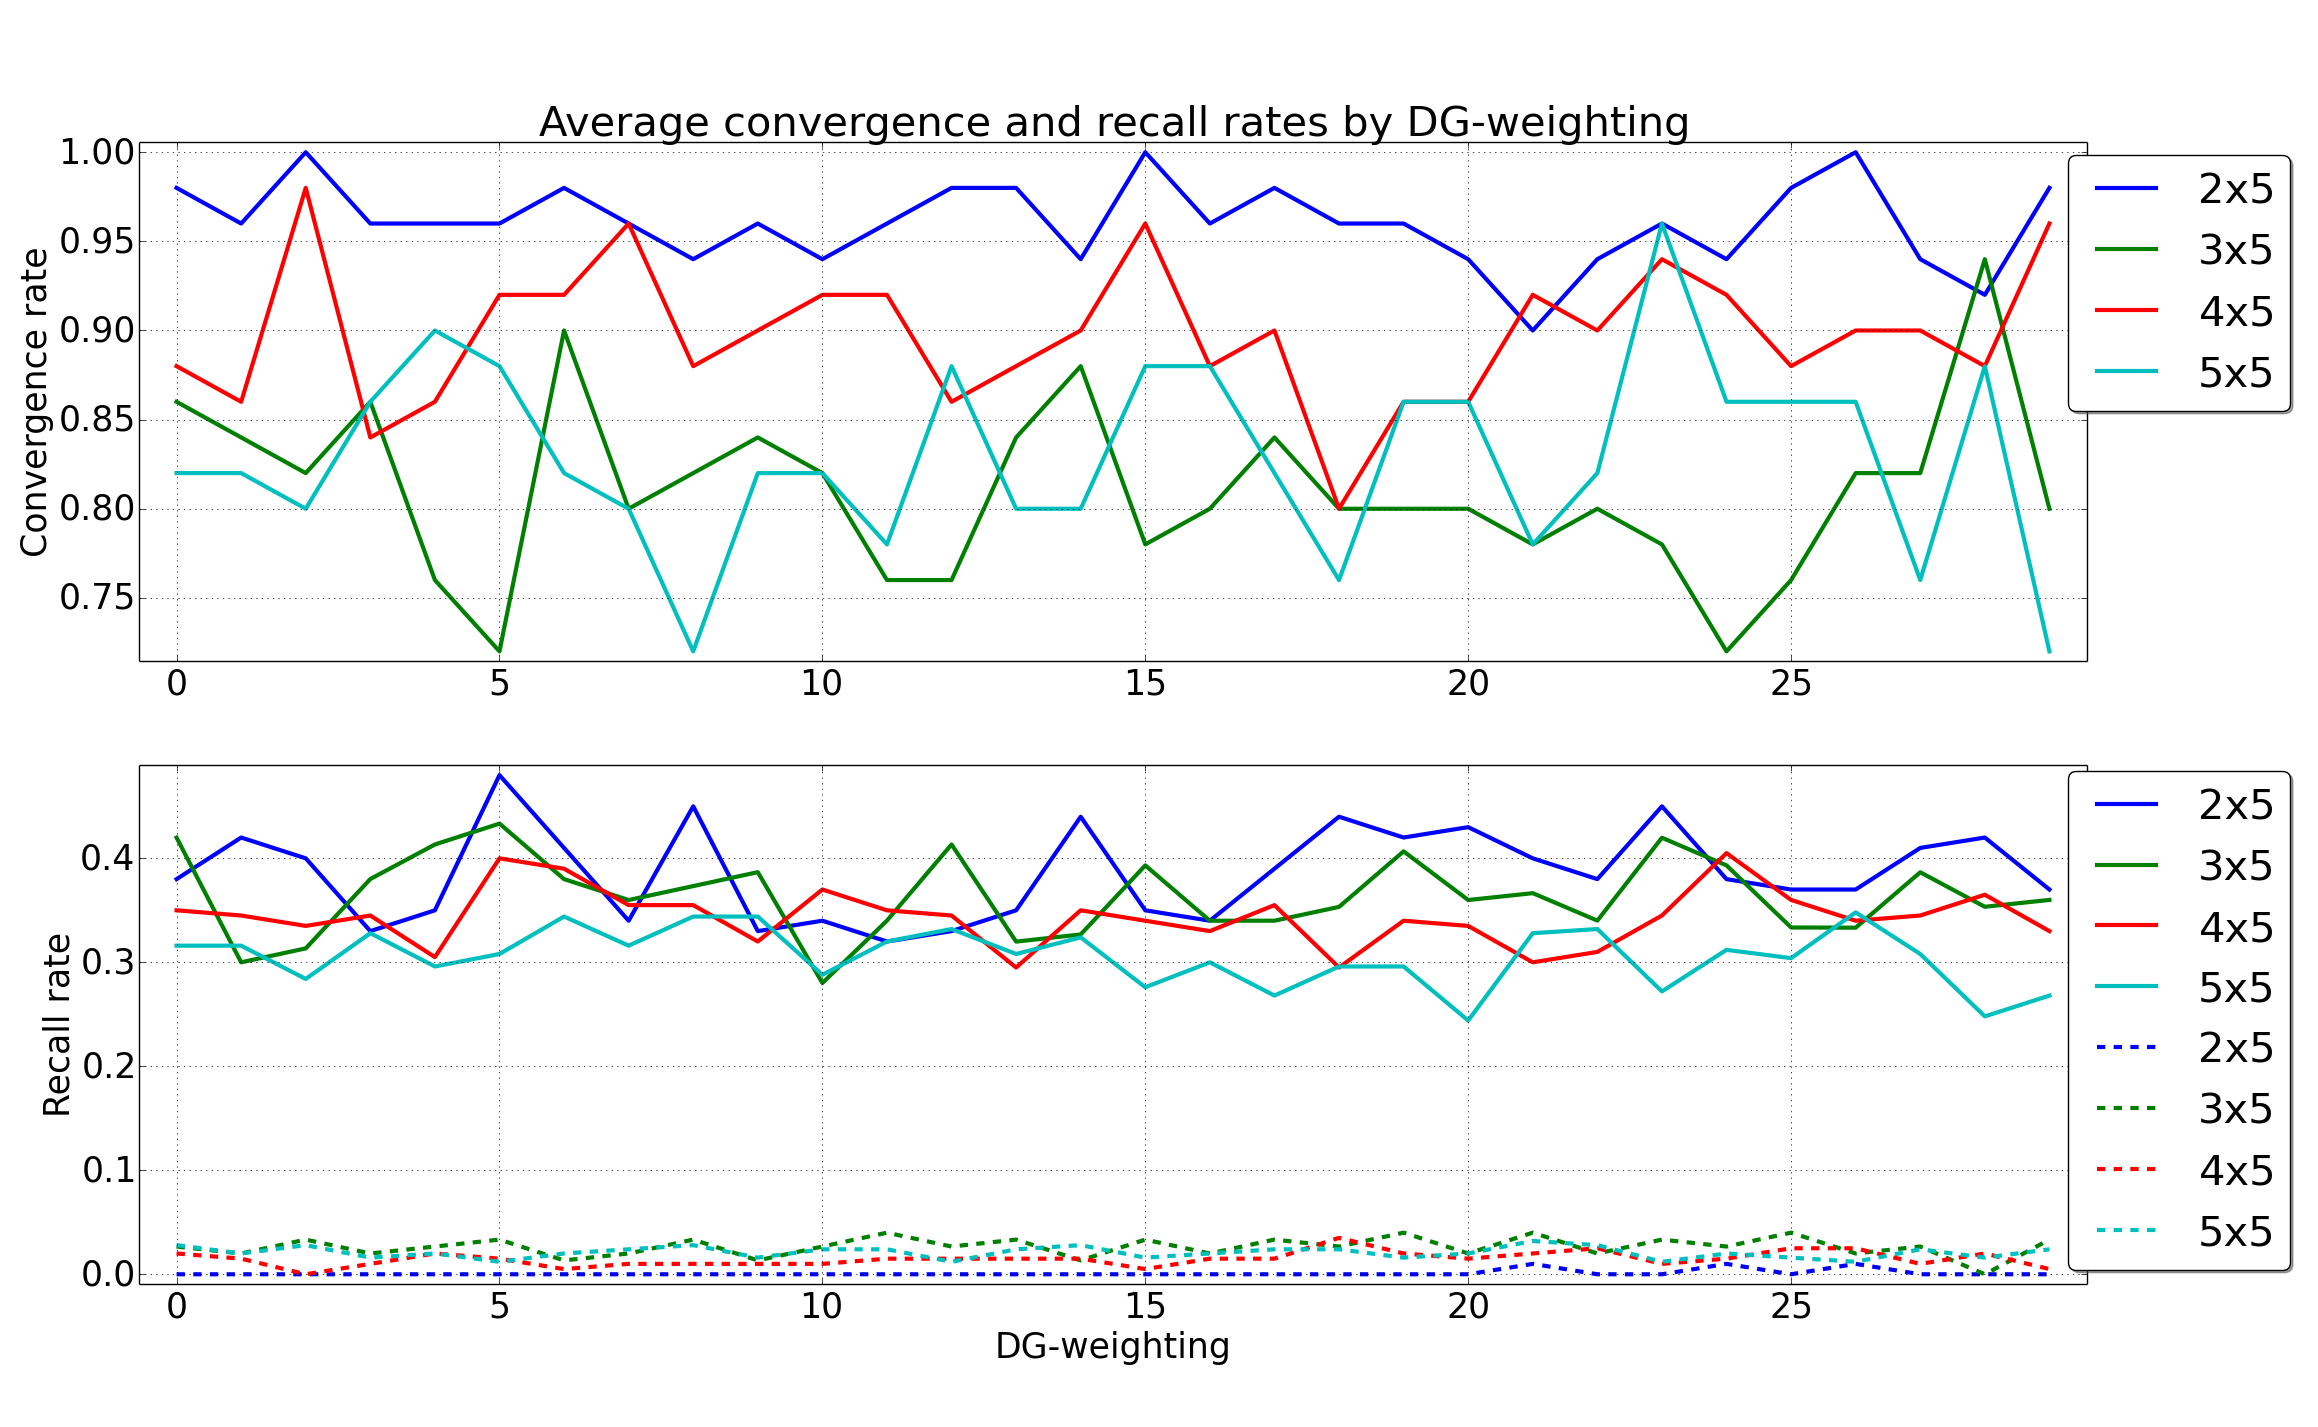
\includegraphics[width=13cm]{fig/DGWs/sync_tm1_04}
    \caption{Showing the results attained for convergence and recall rates by the DG-weighting when using synchronous CA3-layer updating and neuronal turnover for every training iteration, $\tau=0.04$.}
    \label{fig:sync_tm1_04}
\end{figure}

\begin{figure}
    \centering
    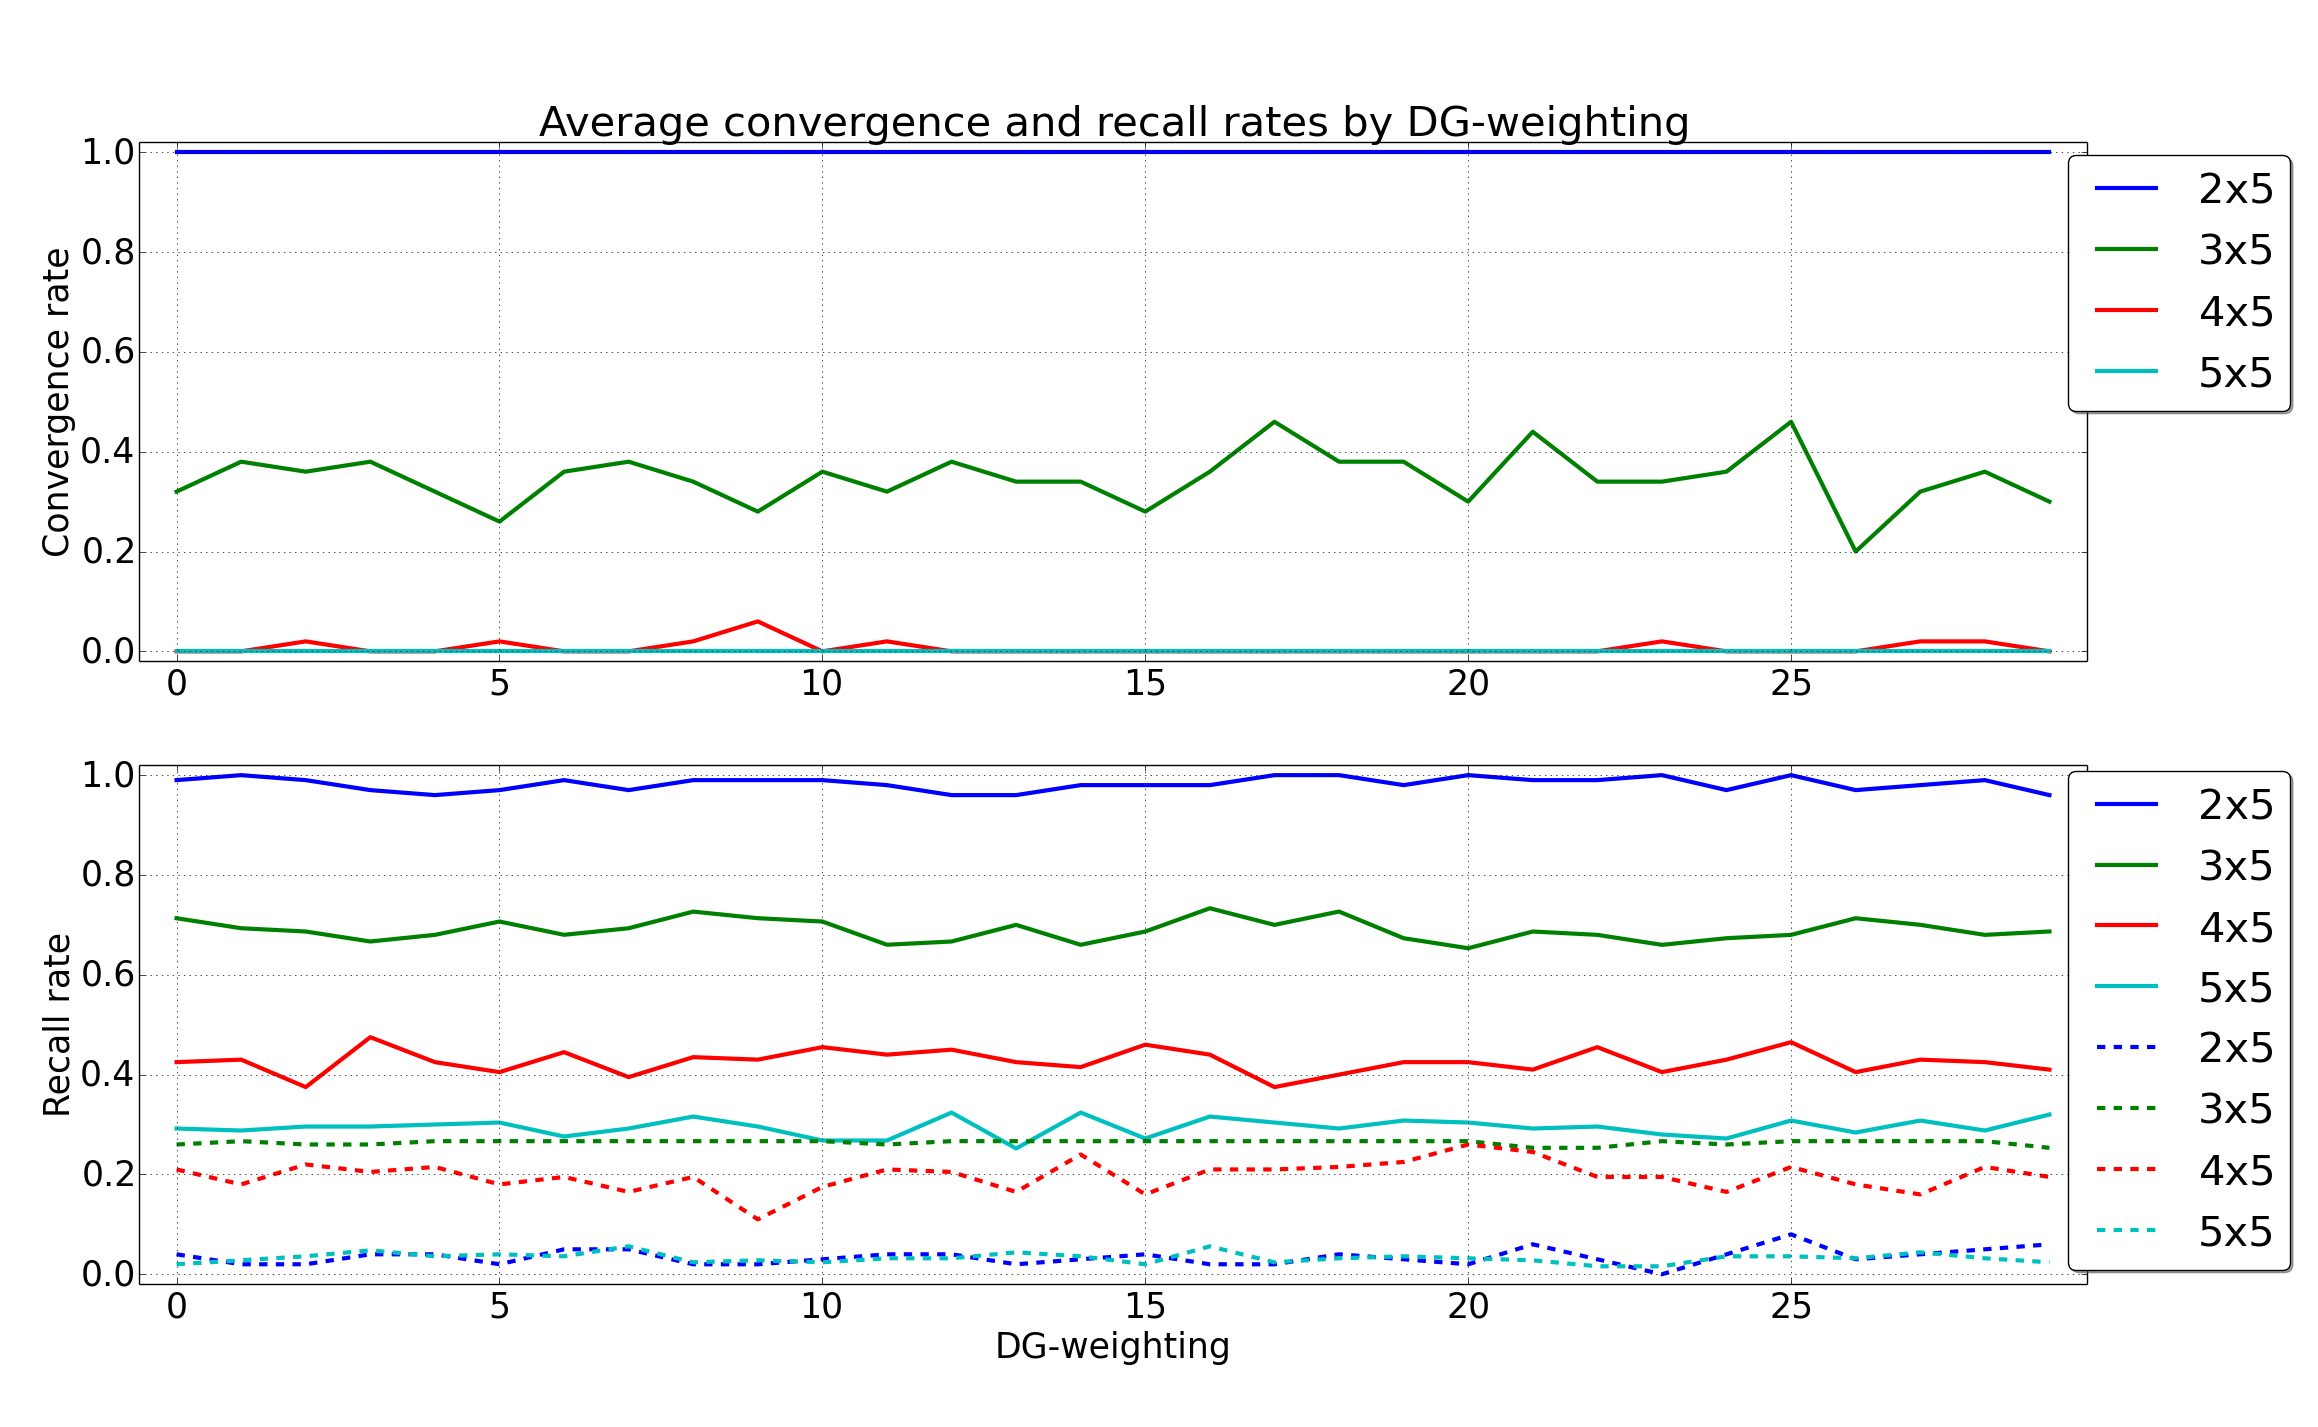
\includegraphics[width=13cm]{fig/DGWs/async_tm1_04}
    \caption{Showing the results attained for convergence and recall rates by the DG-weighting when using asynchronous CA3-layer updating and neuronal turnover for every training iteration, $\tau=0.04$.}
    \label{fig:async_tm1_04}
\end{figure}

\subsection*{Further experiment 4.3 figures: Neuronal Turnover Rates}

\begin{figure}
    \centering
    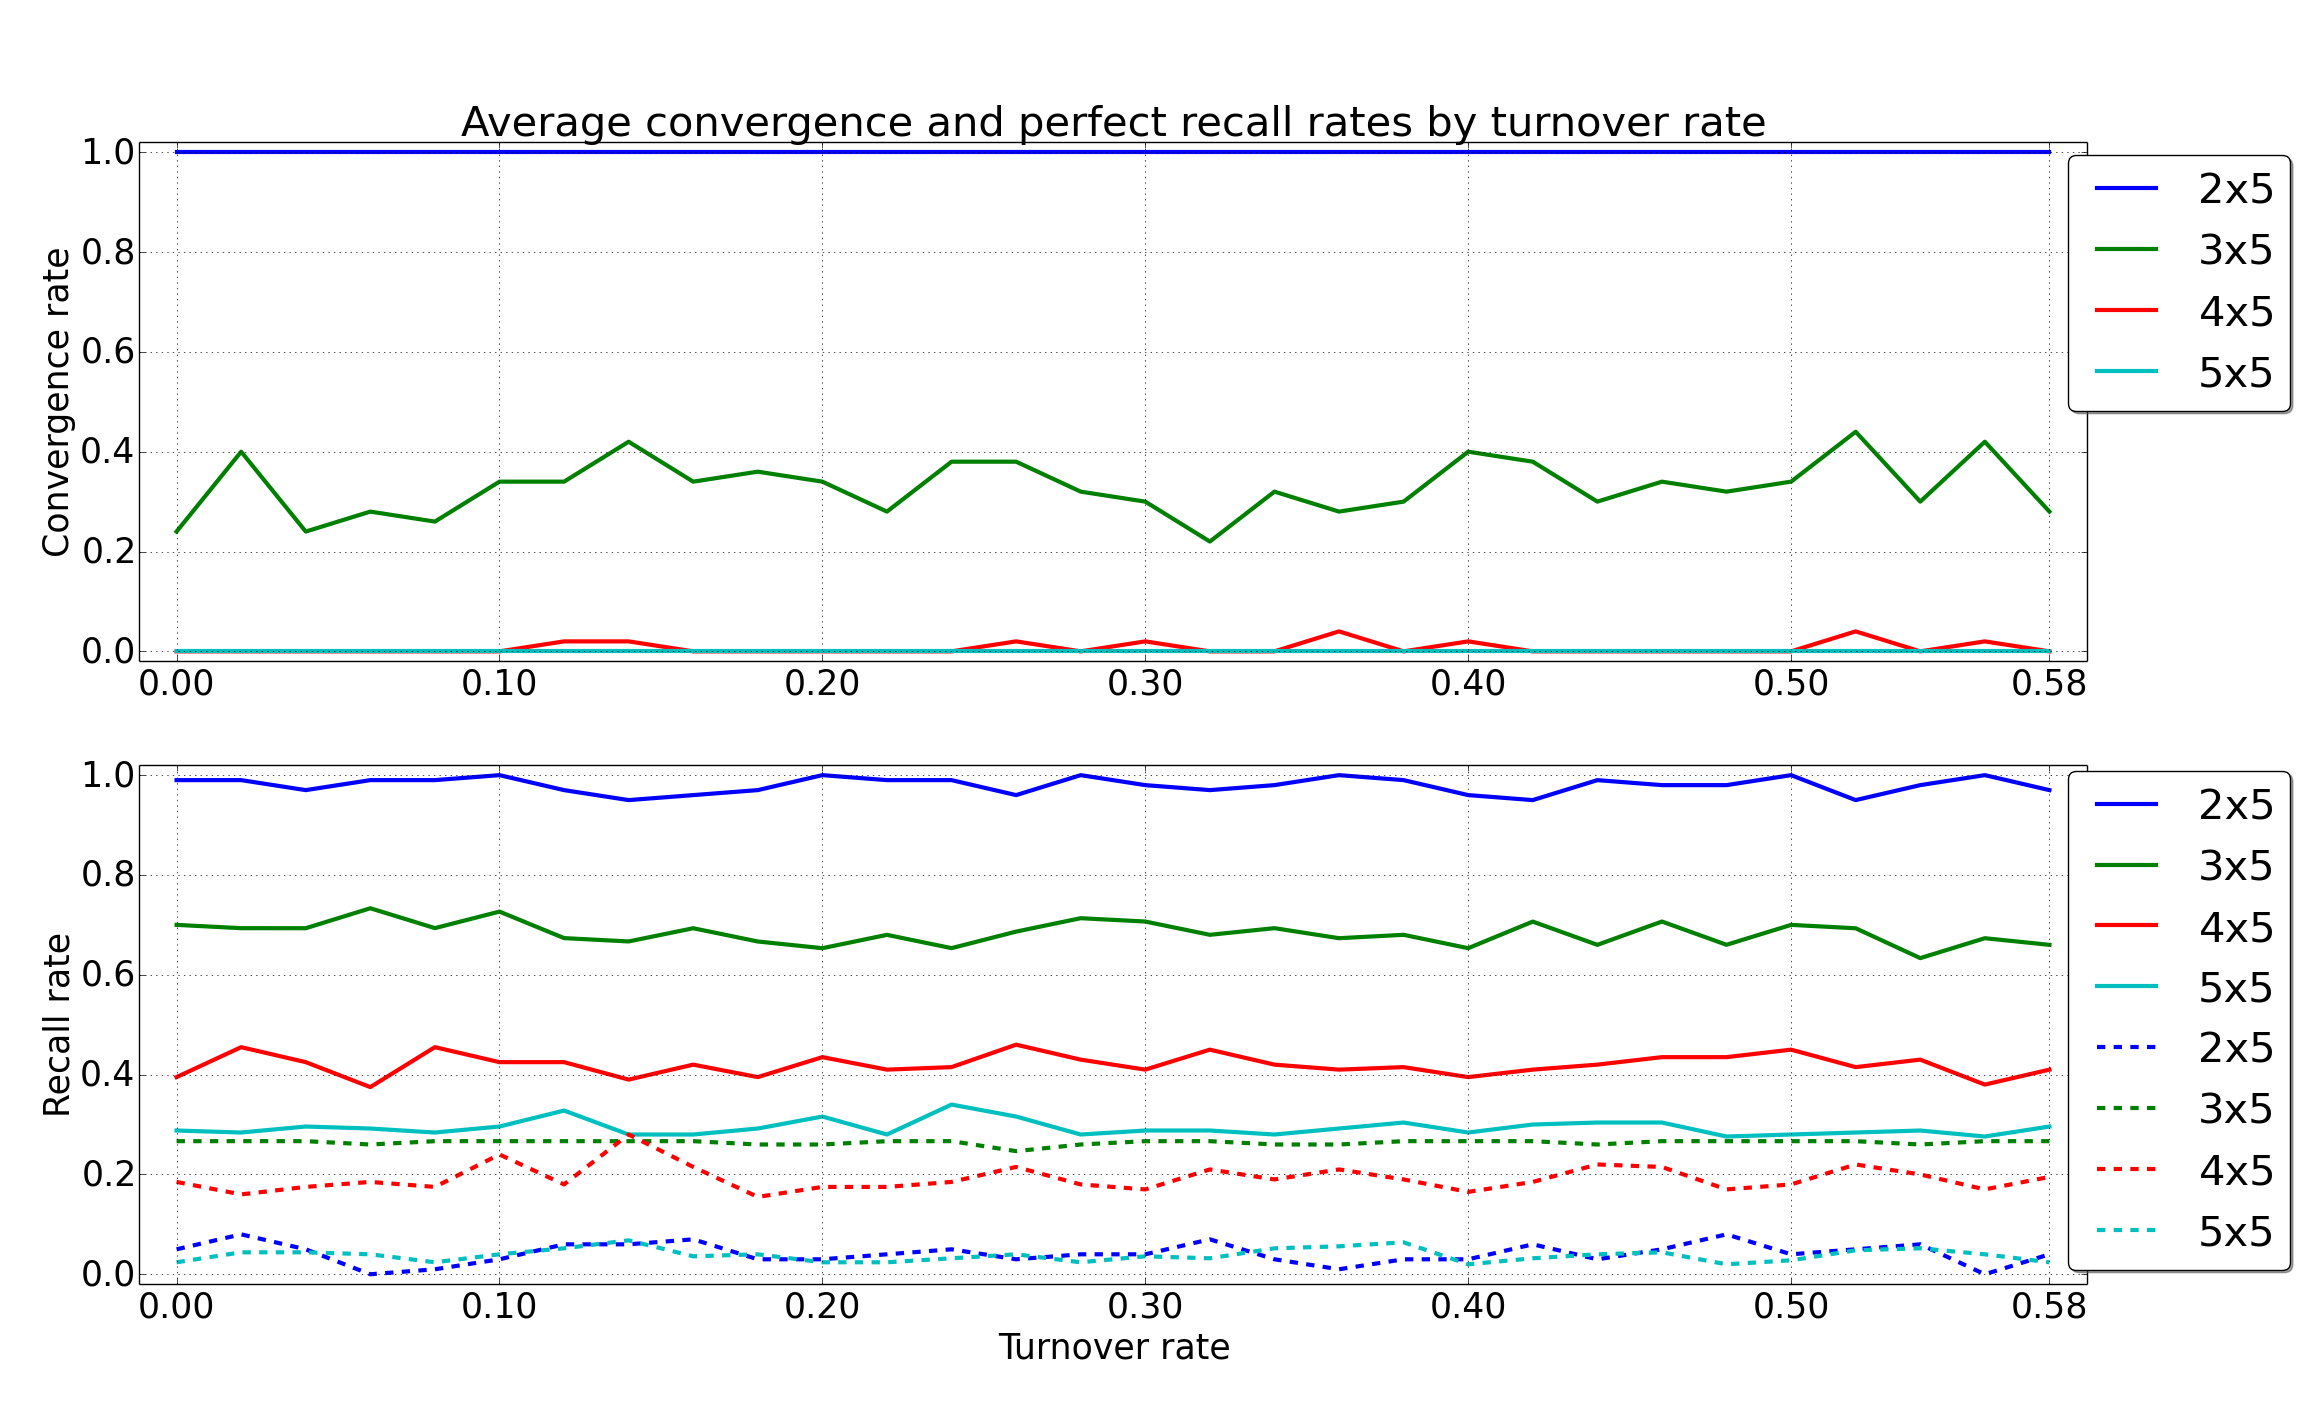
\includegraphics[width=13cm]{fig/turnover_rates/async_tm0_dgw25}
    \caption{Displaying the average convergence- and perfect and spurious recall rates by the neuronal turnover rate for asynchronous CA3-updating, using a DG-weighting of 1, and turnover between every learnt training subset, with $\tau=0.50$.}
    \label{fig:async_tm0_dgw25}
\end{figure}

\begin{figure}
    \centering
    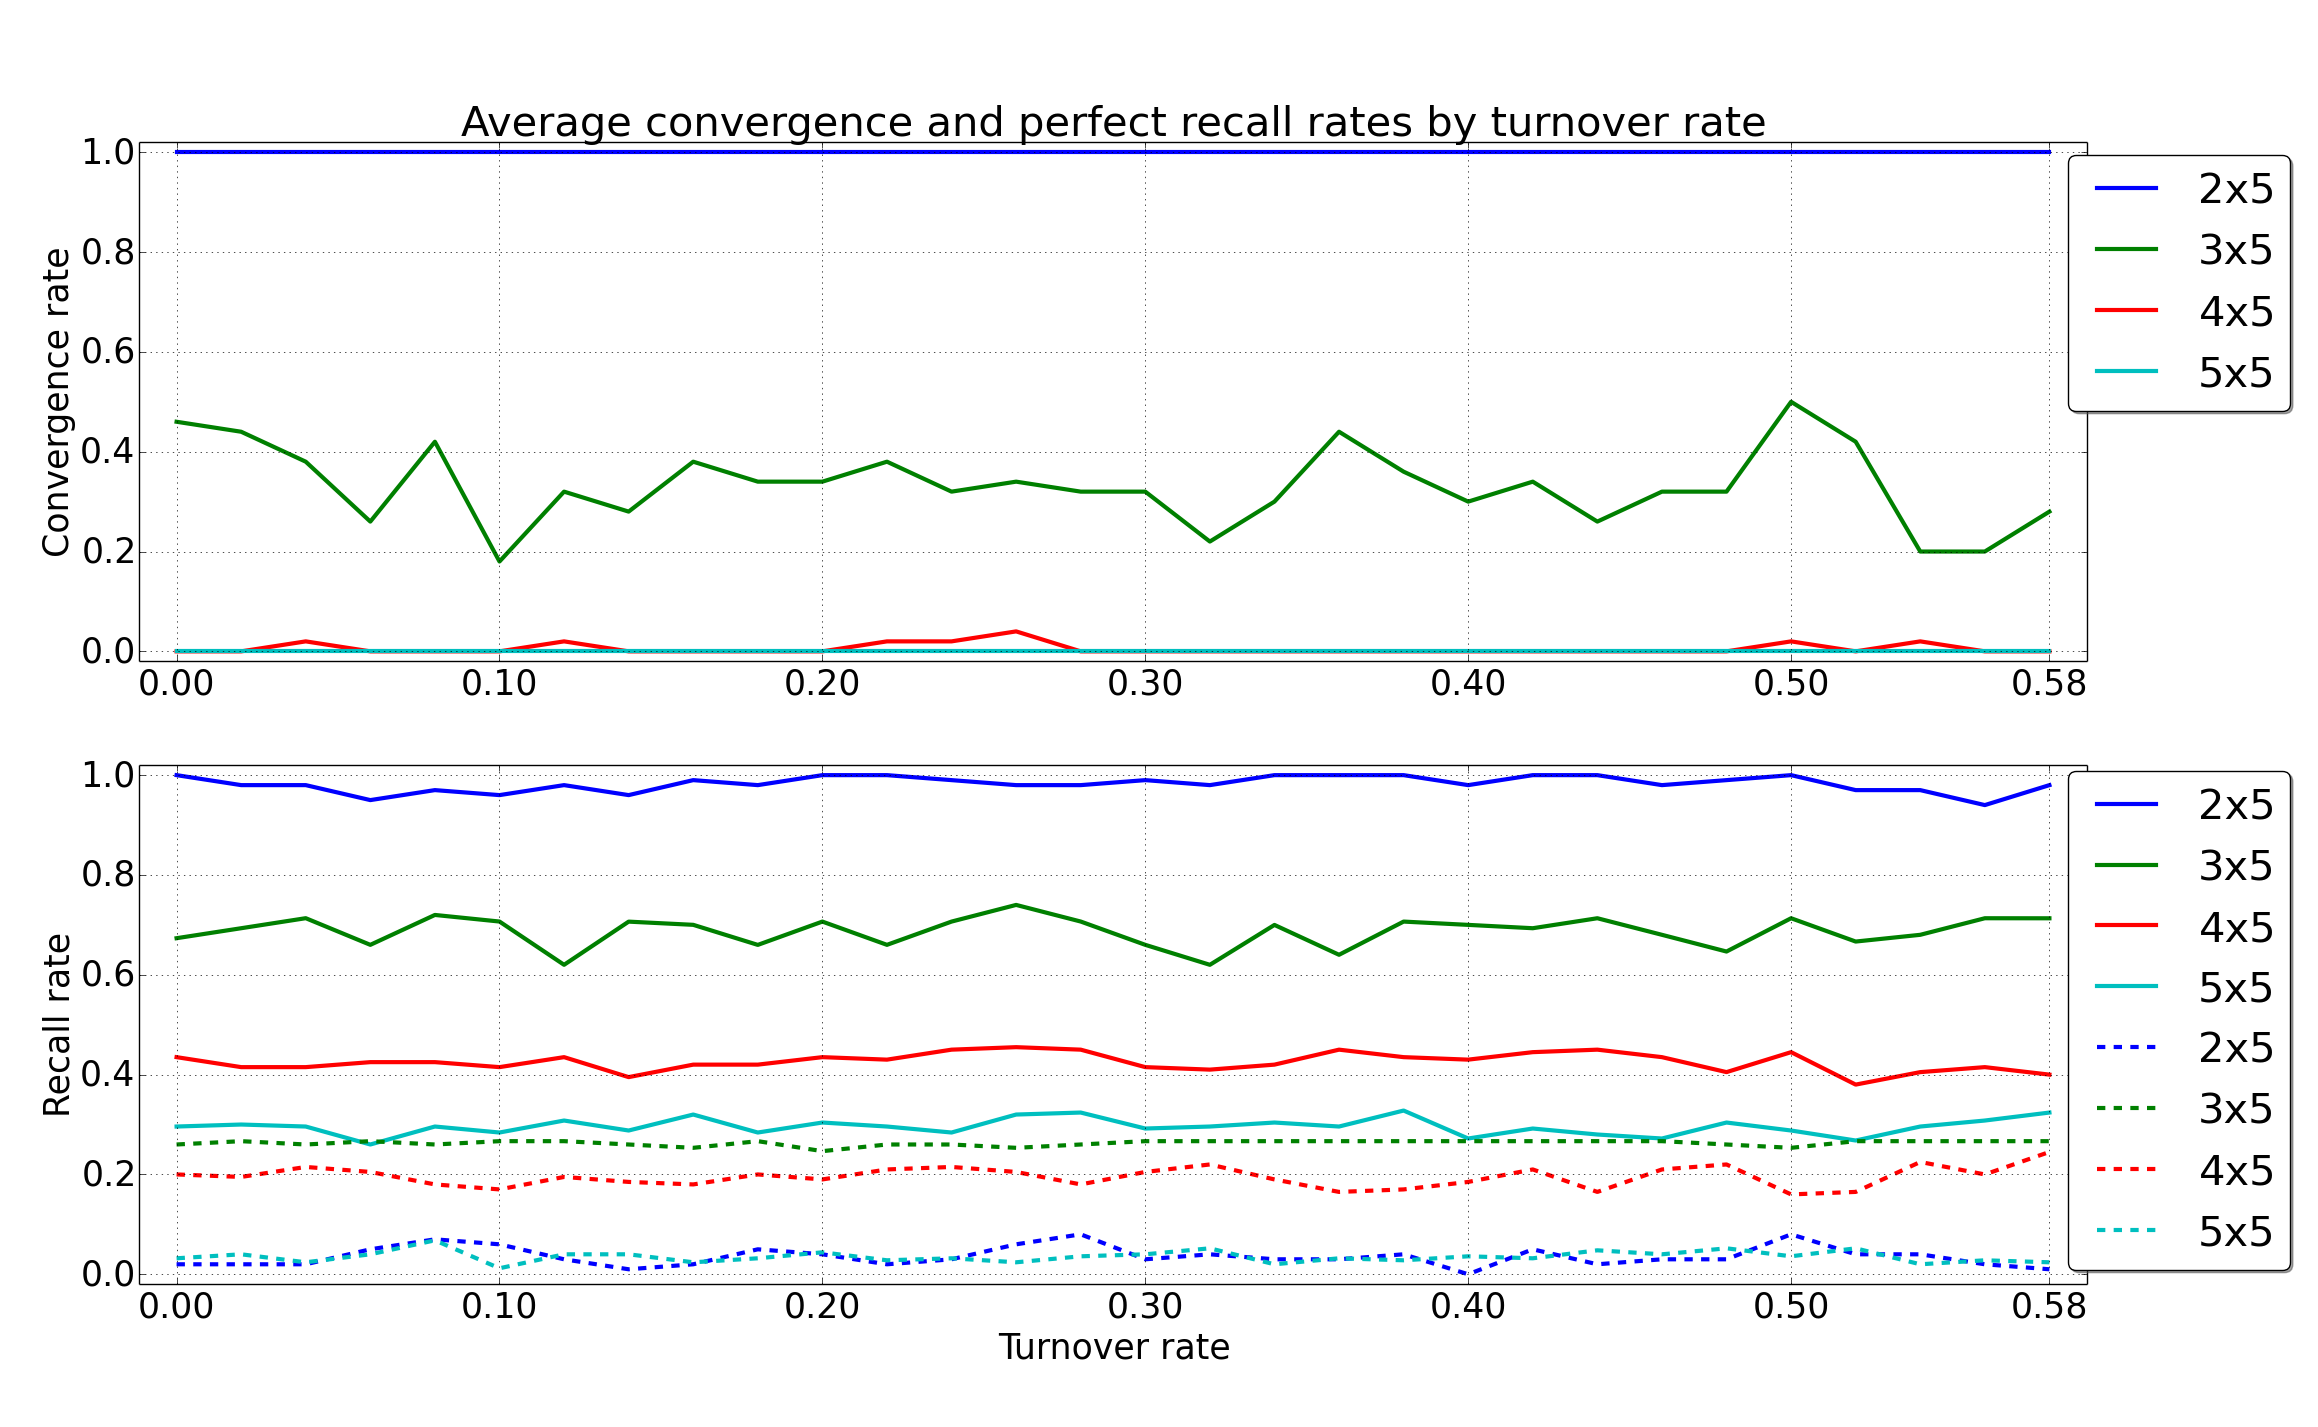
\includegraphics[width=13cm]{fig/turnover_rates/async_tm1_dgw1}
    \caption{Displaying the average convergence- and perfect and spurious recall rates by the neuronal turnover rate for asynchronous CA3-updating, using a DG-weighting of 1, and turnover for every training iteration, $\tau=0.04$.}
    \label{fig:async_tm1_dgw1}
\end{figure}